\documentclass[12pt,letterpaper,english,bibliography=totocnumbered, abstract=on]{scrartcl}

\usepackage[page,toc,titletoc,title]{appendix}


\usepackage{indentfirst}
\usepackage[titletoc]{appendix}
%\usepackage{fullpage}
%\usepackage{subfiles}
\usepackage[T1]{fontenc}
\usepackage[latin9]{inputenc}
\usepackage{color}
\usepackage{babel}
\usepackage{verbatim}
\usepackage[unicode=true,pdfusetitle,
bookmarks=true,bookmarksnumbered=false,bookmarksopen=false,
breaklinks=true,pdfborder={0 0 0},pdfborderstyle={},backref=false,colorlinks=true]
{hyperref}
\hypersetup{linkcolor=blue,citecolor=blue,urlcolor=blue}

\usepackage{booktabs}
\usepackage{multirow}
\usepackage{adjustbox}
\usepackage{threeparttable}
\usepackage[table]{xcolor}
\usepackage{csquotes}
\usepackage{soul} % for hiliting text: \hl

\usepackage[backend=biber, sorting=none]{biblatex}
\addbibresource{CRB.bib}
\addbibresource{extra.bib}

\usepackage{pdfpages}
\usepackage{float} % Allows use of H to place floats

\usepackage{pgfgantt}

\usepackage{framed}
\usepackage{todonotes}

\usepackage{gensymb}

% Prevent page breaks within paragraphs
% https://tex.stackexchange.com/questions/21983/how-to-avoid-page-breaks-inside-paragraphs
\widowpenalties 1 10000


\begin{document}

\titlehead{Final Report: USFS 20-DG-11052021-227}

\title{Improving Coconut Rhinoceros Beetle Breeding Site Detection Using Harmonic Radar}

\author{Aubrey Moore PhD\\University of Guam College of Natural and Applied Sciences}

%\date{January 30, 2023}

\maketitle

\begin{description}
	\item[Federal ID] 20-DG-11052021-227
	\item[Reporting period] 2020-06-17 through 2022-12-31
\end{description}


%\begin{footnotesize}	
%	\url{https://github.com/aubreymoore/2020-FS-CRB-biocontrol-project/raw/master/fs-report-202212/fs-report-202212.pdf}
%\end{footnotesize}

\clearpage

\tableofcontents

\clearpage

\section*{Summary}
\noindent
%\begin{description}
	
%\paragraph{Project Staff}
%	The project's insect pathologist, Dr. James Grasela retired during June 2022. Prior to leaving, he produced 2 presentation posters to document some of his research results \cite{graselaPreliminaryDetectionWolbachia2022,graselaPreliminaryEffortsEstablish2022}. The latter poster was presented at the Annual Meeting of the Entomological Society of America, Vancouver in November 2022. The project currently supports a full time technician, Christian Cayanan and three part time student research assistants. Laura Caser, Raimunt Mesubed and LeahMarie Bukurou. Raimunt and LeahMarie previously worked on CRB research in Palau under Dr. Chris Kitalong.
%	
%\paragraph{Laboratory Activities}
%	We have established a CRB rearing facility to rear high quality, disease free CRB adults to be used in laboratory bioassays. We have developed a natural larval diet by sterilizing material from dead standing coconuts \cite{Moore_Caser_Cayanan_Mesubed_2023}. We are currently testing CRB gut samples from Palau to see if they contain Oryctes nudivirus which can be used as an effective biological control agent for CRB-G on Guam \cite{Moore_Caser_2023}.
%	
%\paragraph{Field Activities}	
%	We continue to run island-wide roadside surveys to monitor CRB damage to coconut palms on Guam. We also maintain pheromone traps as a source of CRB adults for our rearing program and for experiments.
%	
%\paragraph{Pacific Ecological Security Conference (PESC)}	
%	 Project resources were used in support of the PESC which was held in Palau during September 2022. The PI participated in preparatory teleconferences and preparation of a strategic action plan for responding to CRB on Pacific Islands. The PI attended the conference in Palau as an invited delegate from Guam during which he helped finalize the CRB strategic action plan \cite{anonymousCoconutRhinocerosBeetle2022}. He also attended a meeting convened by the Office of Insular Affairs and the Forest Service at which he made a short presentation on the status of invasive species on Guam \cite{mooreOverviewInvasiveSpecies2022}.

%\newpage
%
%\subsection*{Notes for the Reader}
%
%\begin{itemize}
%
%\item Each objective, as stated in the funded grant proposal \cite{mooreGrantProposalDOIOIA2020}, is presented in a frame at the start of each of the following sections. 
%
%\item The University of Guam CRB biological control project is a long-term effort supported by multiple short-term grants.  
%
%\end{itemize}
%
%\clearpage
%
%\section{Objective 1: Survey to Determine Background OrNV Incidence} 
%
%\begin{framed}
%CRB adults collected from breeding sites and pheromone traps throughout Guam will be tested for presence of OrNV using PCR.  Laboratory bioassays will be performed on OrNV isolated from these beetles to evaluate potential for biological control.
%\end{framed} 
%
%\subsection{Previously reported progress}
%
%Our lab currently uses CRB-G adults collected from pheromone traps as test animals in bioassays to evaluate OrNV isolates as biocontrol agents under the assumption that the Guam beetle population contains only the CRB-G biotype and is free from OrNV infection. In 2019 we gained the capacity to perform PCR in our lab and began testing these assumptions. PCR results indicated that untreated, field-collected beetles, used as experimental controls in our bioassays, were all CRB-G, but 18\% of these tested positive for OrNV \cite{graselaTechnicalReportPolymerase2020, graselaTechnicalReportPolymerase2020a}.
%
%Based on these results, the PI decided to suspend bioassays until we had conclusive evidence of OrNV infection in the Guam CRB-G population.  This decision was made for two reasons:
%
%\begin{enumerate}
%	\item If field-collected CRB insects where already infected with OrNV, these could not be used as test insects in laboratory bioassays designed to evaluate virulence of OrNV isolates.
%	\item If an OrNV strain was already spreading within the Guam CRB population, it would be prudent to evaluate this strain as an effective biological control agent. 
%\end{enumerate}
%
%An experimental plan \cite{mooreExperimentalPlanDetermining2020} was developed and executed. One hundred beetles were collected from each of two pheromone trapping sites (Leo Palace Resort in Southern Guam and the UOG Ag. Expt. Stn. in northern Guam). Gut samples were obtained from these beetles and tested using PCR in our lab and also in Sean Marshall's lab at AgResearch New Zealand. 
%
%In PCR results from both labs all beetles tested positive for CRB-G biotype and negative for OrNV infection \cite{graselaInvestigationDeterminePresence2020}. 
%
%We concluded that previous OrNV positive tests were the result of lab contamination (not false positives). 
%
%Current evidence suggests that all CRB on Guam belong to the CRB-G biotype and there is no OrNV infection within this population. In other words, the background OrNV incidence is zero.
%
%\subsection{Recent progress}
%
%Work on this objective has been completed. All evidence indicates that the OrNV incidence in the Guam CRB population is zero. We concluded that previous OrNV positive tests were the result of contamination in our lab. We have improved protocols to address this problem.
%
%\clearpage
%\section{Objective 2: Establish Sustainable CRB-G Biocontrol by Autodissemination of OrNV}
%
%\begin{framed}
%		
%OrNV biocontrol candidates will be propagated \textit{in vivo} using established methods \cite{huger_oryctes_2005-1} and released into the Guam CRB-G population by autodissemination. Autodissemination involves infecting healthy CRB adults with OrNV. These infected beetles are then released at points dispersed throughout the island where they vector disease to conspecifics. A permit for field release of OrNV on Guam has already been obtained from USDA-APHIS. All released beetles will be marked by etching unique numbers on their elytra using a computer-controlled laser engraving system system already in use for this application at UOG.
%
%Beetles for \textit{in vivo} propagation of OrNV and autodissemination will be field-collected from breeding sites and pheromone traps because this is far more efficient than rearing beetles in the lab at the current time. Impact of virus releases will be monitored using pheromone traps and a novel roadside video analysis system (see Objective \ref{monitoring}). A subset of beetles captured in traps will be used to estimate the virus infection rate. Concurrent with virus releases, we will continue to screen OrNV isolates to find candidate biocontrol agents.
%\end{framed}
%
%\subsection{Previously reported progress}
%
%We have not made progress on this objective for two reasons:
%\begin{enumerate}
%	\item High mortality of untreated insects in experimental control groups and discovery of OrNV in some of these insects, presumably from laboratory contamination, have thrown results of previous bioassays into question.  We need to re-test several OrNV isolates we have previously evaluated in laboratory bioassays.
%	\item We require permission from the US Environmental Protection Agency (USEPA) prior to release of OrNV as a biological control agent. Data demonstrating efficacy of OrNV as a biological control agent is required by USEPA.  
%\end{enumerate}
%
%We are currently reviewing our lab methods before resuming laboratory bioassays of OrNV isolates. We are considering changes to minimize OrNV contamination of samples in the bioassays and re-establishment of a CRB rearing program to provide high-quality test insects instead of relying on field-collected beetles.
%
%\subsection{Recent progress}
%
%We have revised our laboratory bioassay protocols. Previously, we used adults collected from pheromone traps as test insects. This source did not produce high quality, standardized adults needed for bioassays because these beetles were of unknown age and some were infected with pathogens or had other health problems. This caused high variability and high experimental control group mortality in our bioassay results. We now rear CRB from egg to adult in a dedicated CRB rearing lab using a natural diet we have developed. Adults produced by this lab are healthy, pathogen free and of a known age.
%
%\paragraph{Development of a natural diet for CRB rearing.}
%
%Previously, we individually reared CRB from egg to adult by placing them in Mason jars filled with a commercial steer manure/soil blend purchased from local hardware stores. However this is risky because manure may contain persistent pesticides fed to cattle or pesticides applied to the manure for fly control. 
%
%We decided to eliminate this risk by making our own rearing diet from dead standing coconut stems which have begun to rot. We preferentially harvested stems naturally infested CRB grubs.
%
%Processing is simple:
%\begin{enumerate}
%	\item Dead standing coconut stems are felled and bucked into 4 foot lengths
%	\item Logs are run through a chipper and chips are loaded into burlap bags. Bags are placed in a chest freezer until needed.
%	\item Chip size is reduced in an industrial Waring blender
%	\item Material is loaded into Mason jars. This filled jars are sterilize using an autoclave
%\end{enumerate}
%
%\paragraph{Establishment of a CRB rearing lab.}
%
%We converted a 40 foot shipping container into a CRB rearing lab. Temperature is maintained at 80\degree F by two independent air conditioners. Insects are reared individually from egg to adult by placing them in Mason jars filled with a natural rearing medium made from chipped standing dead coconut stems. There is shelf space for more than 2,000 jars (Fig. \ref{fig:rearing-lab}).
%
%% TODO: \usepackage{graphicx} required
%\begin{figure}[h]
%	\centering
%	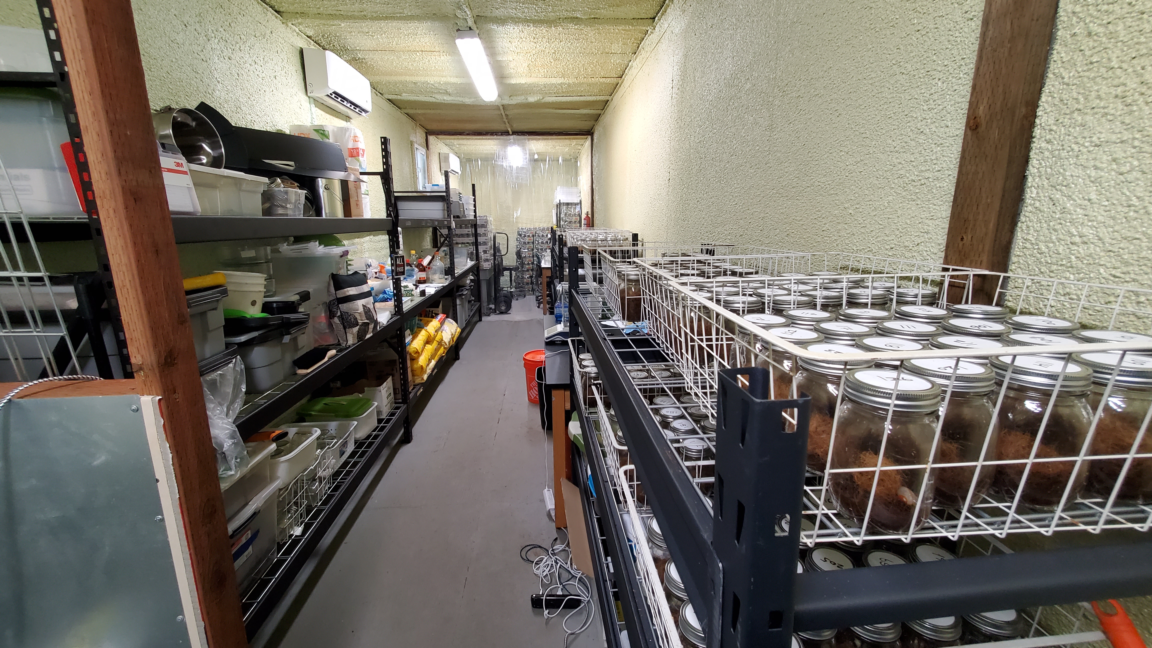
\includegraphics[width=\linewidth]{images/rearing-lab}
%	\caption{Coconut rhinoceros beetle rearing lab at the University of Guam.}
%	\label{fig:rearing-lab}
%\end{figure}
%
%
%\paragraph{Bioassays to determine sublethal effects of OrNV.}
%
%Sublethal affects of OrNV infection may be much more important for CRB population suppression than direct mortality. A lab bioassay reported by Prasad et al. 2008 \cite{prasadManagementCoconutRhinoceros2008} showed that a high dosage of OrNV reduced the number of eggs laid per female from a mean of 58.5 to zero (100\% reduction in fecundity). Remarkably, when this dosage was reduced by a factor of 1000, the number of eggs laid per female was reduced from a mean of 58.5 to 16.5 (71.8\% reduction in fecundity).
%
%We are preparing to repeat thus experiment using OrNV isolate V23B against CRB-G adults produced by our rearing lab. Isolate V23B is of particular interest because this isolate has been shown to infect CRB-G by our lab and also by independent research with CRB-G in the Solomon Islands \cite{barreraElectronMicroscopyStudy2021}. 
%
%If the V23B isolate significantly reduces fecundity, we will use the results as evidence of efficacy as required by the US Environmental Protection Agency in support of a field application permit.
%
%Our rearing facility is now starting to produce adults and bioassays will begin soon.
%
%\clearpage
%
%\section{Objective 3:  Establish Island-wide Monitoring Systems for CRB and Coconut Palm Health}
%\label{monitoring}
%
%\begin{framed}
%The CRB-G outbreak on Guam is currently unmonitored on an island-wide basis. An island-wide pheromone trapping system, using about 1500 traps, was operated by the University of Guam from 2008 to 2014. This monitoring system was transferred to the Guam Department of Agriculture which abandoned the effort at the end of February, 2016.  Currently, many coconut palms are being killed by CRB-G. But, in the absence of a monitoring system, we do not have an estimate of tree mortality or whether or not the damage is increasing or decreasing. Clearly, establishment of a monitoring system is necessary to evaluate success of the proposed biocontrol project, or any other mitigation efforts. We intend to re-establish island-wide trapping and to establish a sustainable roadside video survey which uses artificial intelligence to detect CRB damage in dash-cam videos. 
%\end{framed}
%
%\subsection{Objective 3a: Pheromone Traps}
%
%%\begin{framed}
%%We plan to installed 150 CRB pheromone monitoring traps. These will be baited with oryctalure and serviced semimonthly. These traps catch approximately equal numbers of males and females which remain alive in the traps for several weeks. Collected beetles will be used for autodissemination of virus and a subsample will be used for virus detection. Traps will be deployed at least 3 months prior to initiation of autodissemination.  
%%
%%A web database already exists for Guam CRB trap data and it is available for use by this project (URL: \url{https://mysql.guaminsects.net}; database: \textbf{oryctes}; user: \textbf{readonlyguest}; password: \textbf{readonlypassword}; main tables: \textbf{trap} (2,265 records) and \textbf{trap\_visit} (89,114 records)).
%%\end{framed}
%
%\subsubsection{Previously reported progress}
%
%We have not deployed new pheromone traps. But we continue to maintain trap lines in central Guam, at the Leo Palace Resort, and in northern Guam, at the University of Guam Agricultural Station in Yigo.
%
%\subsubsection{Recent progress}
%
%We maintain 35 pheromone traps at the Leo Palace Resort Golf Course. These are serviced biweekly. The main purpose of this activity is to provide adult beetles for experiments.
%
%We have decided not to use pheromone traps for island-wide monitoring because we don't know the relationship between trap catch and CRB population density. Mark-release-recapture studies show that the commercially available pheromone, oryctalure, is not highly attractive to CRB-G on Guam \cite{siderhurstEffectsUltravioletLight2021}. The recapture rate for 567 marked beetles released in the vicinity of pheromone traps was only 11\%.
%
%We will continue to use automated roadside image surveys as a cost-effective instead of pheromone traps for island-wide monitoring of CRB on Guam. 
%
%\clearpage
%\subsection{Objective 3b: Roadside Video Surveys}
%
%\begin{framed}
%Damage symptoms such as v-shaped cuts to fronds, bore holes, and dead standing coconut palm stems are readily observed during roadside surveys. Survey data will be collected on a smart-phone dash-cam app which georeferences each image. Initially, images of coconut palm damage by CRB-G will be detected, classified and tagged by a technician. When a large number of images have been tagged, these will be used to train an object detector. This work will result in a fully automated CRB damage detection and monitoring system which generates detection alerts and damage maps. This automated system will be useful as an early detection device for CRB. Roadside surveys on Guam will be performed bimonthly and the system will also be tested on Tinian, an island just north of Guam on which CRB has never been detected.
%
%The envisioned system has already been successfully prototyped. A custom object detector for CRB damage has been trained using the TensorFlow implementation of the Faster R-CNN Deep Learning model (Moore, unpublished).
%\end{framed}
%
%\subsubsection{Previously reported progress}
%
%Bimonthly automated roadside video surveys for CRB damage are now operational on Guam and the system has been tested on Rota. Videos recorded with a smart phone attached to a vehicle are analyzed using custom-designed artificial intelligence software which recognizes coconut palms and measures CRB damage. A nontechnical description of the survey method is given in the next section.
%
%A presentation on this new CRB survey methodology was made at the December 9 2020 meeting of the CRB-G Action Group conducted as a Zoom webinar. Videos of all presentations at this meeting are available online \cite{mooreVideoRecordingCRBG2020}.
%
%\clearpage
%\paragraph{Guam Roadside Video Survey 1}
%
%The following four images were extracted from a draft of the University of Guam's Western Pacific Tropical Research Center impact report for 2020. They provide a nontechnical overview of the new automated roadside video survey for CRB damage and results from the first Guam survey in October, 2020.
%
%\begin{figure}[h]
%	\centering
%	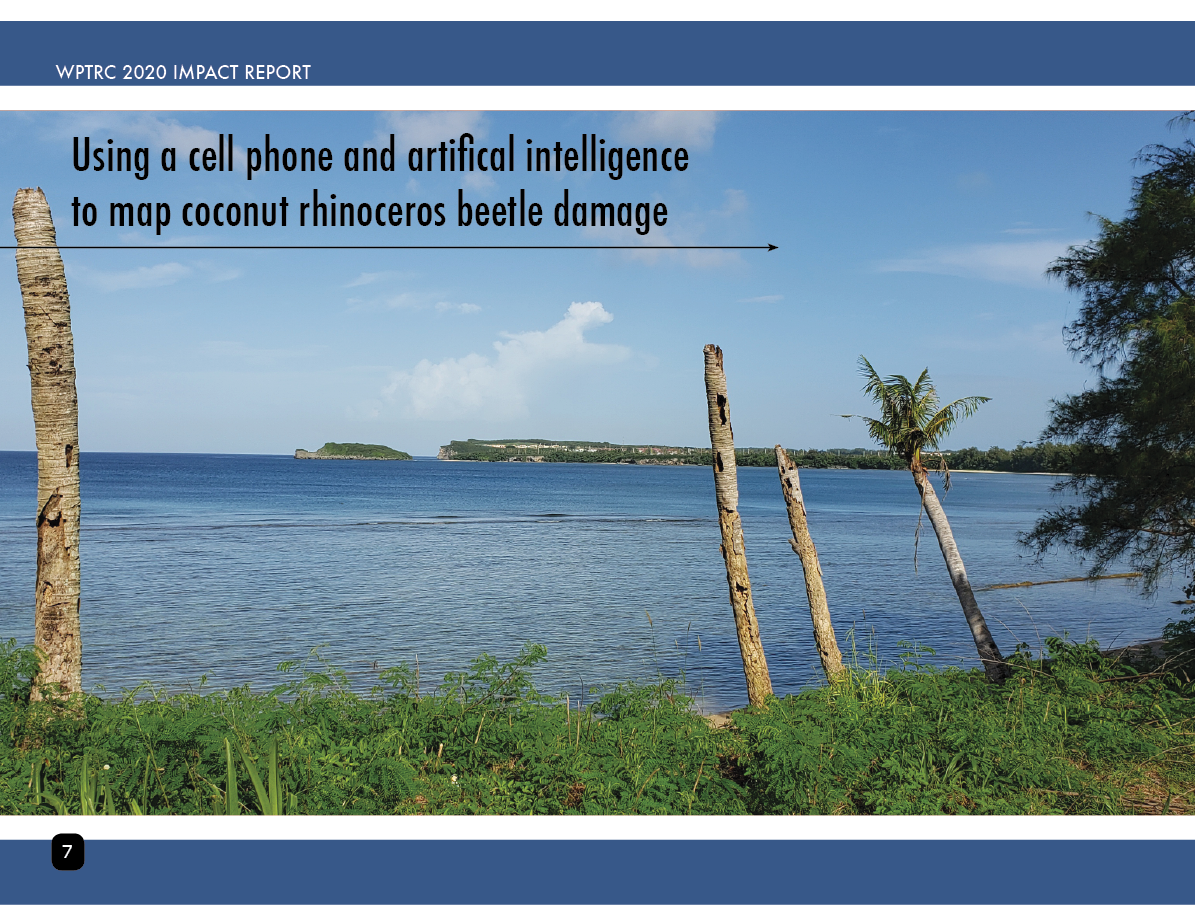
\includegraphics[width=1\linewidth]{images/impact-report07.png}
%	\caption{Feature article in the University of Guam's Western Pacific Tropical Research Center impact report for 2020.}
%	\label{fig:roadside1-1}
%\end{figure}
%
%\begin{figure}[h]
%	\centering
%	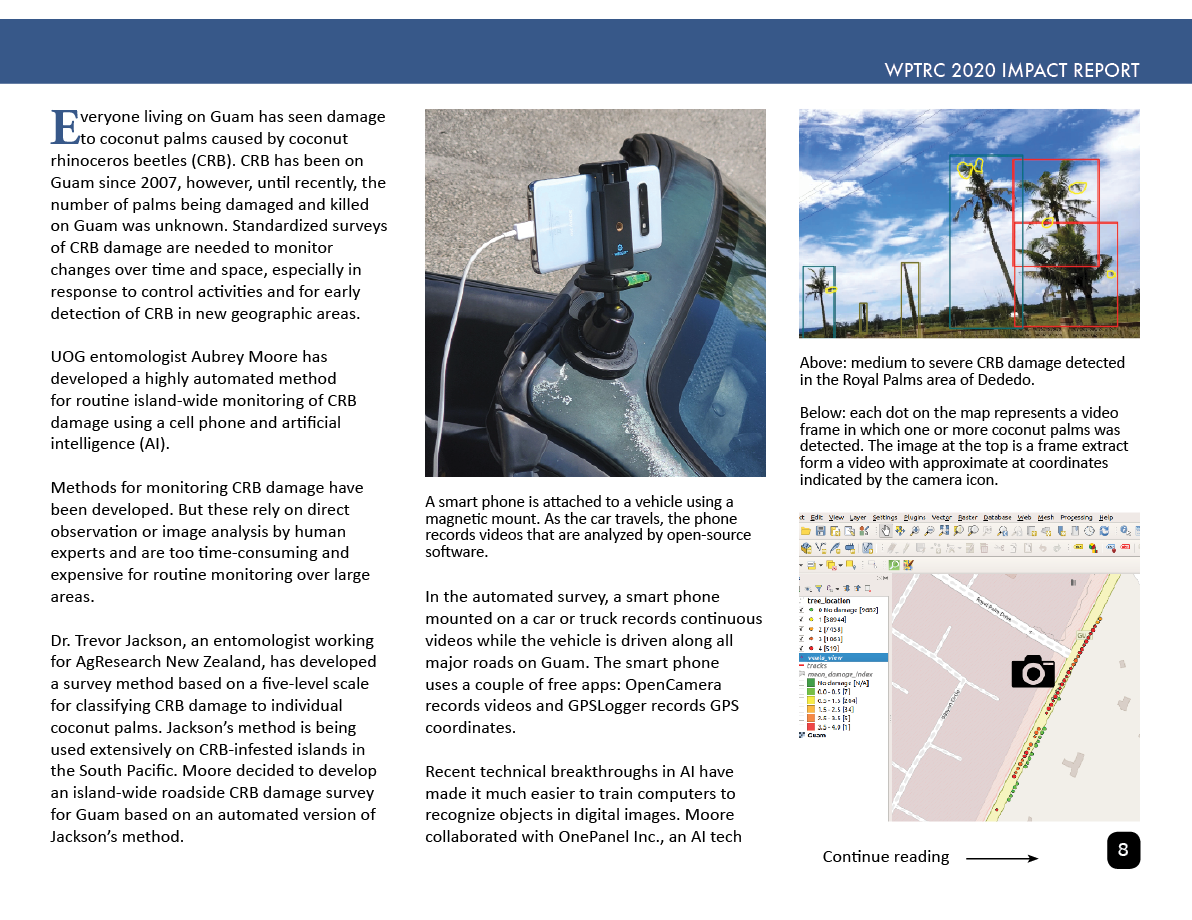
\includegraphics[width=1\linewidth]{images/impact-report08.png}
%	\caption{[Continued] Feature article in the University of Guam's Western Pacific Tropical Research Center impact report for 2020.}
%	\label{fig:roadside1-2}
%\end{figure}
%
%\begin{figure}[h]
%	\centering
%	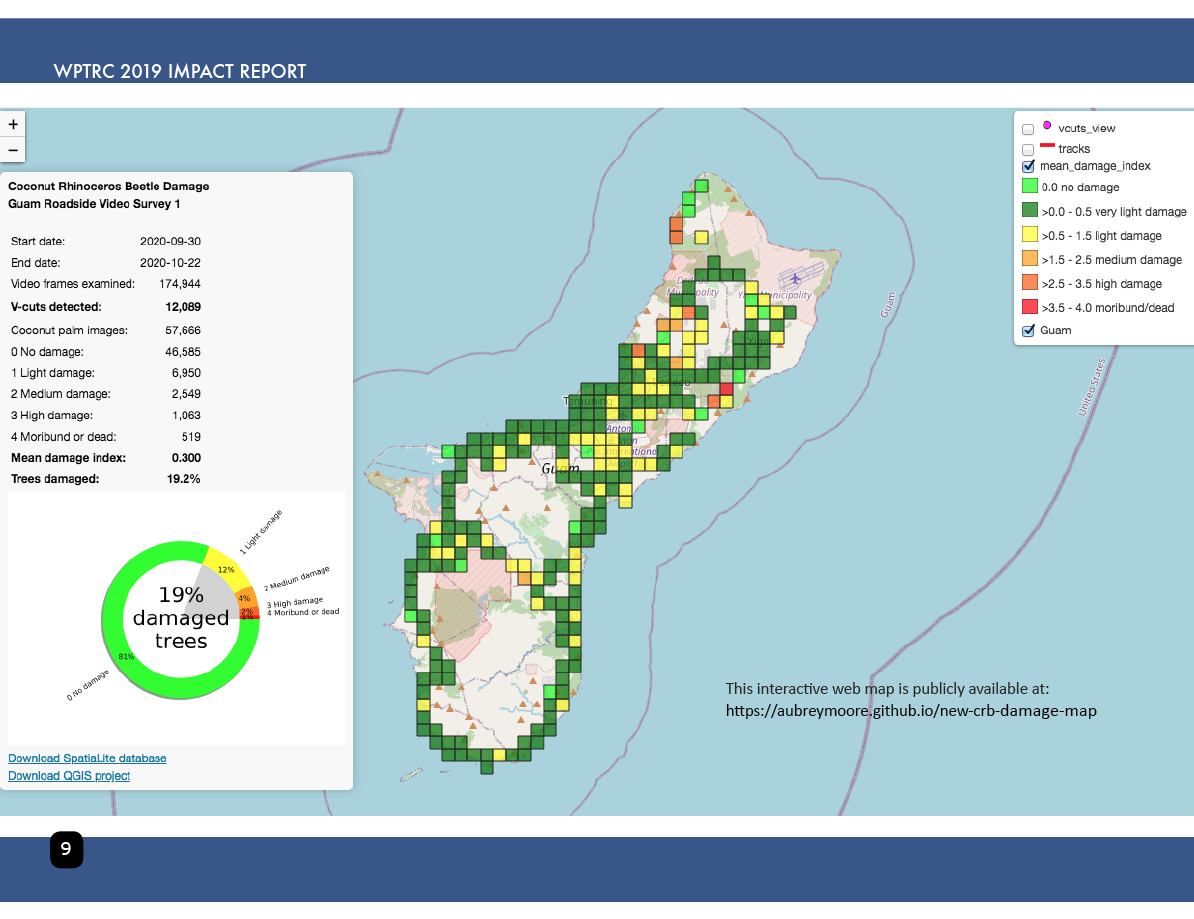
\includegraphics[width=1\linewidth]{images/impact-report09.png}
%	\caption{[Continued] Feature article in the University of Guam's Western Pacific Tropical Research Center impact report for 2020. This interactive web map is publicly avaiable at: \url{https://aubreymoore.github.io/new-crb-damage-map}}
%	\label{fig:roadside1-3}
%\end{figure}
%
%\begin{figure}[h]
%	\centering
%	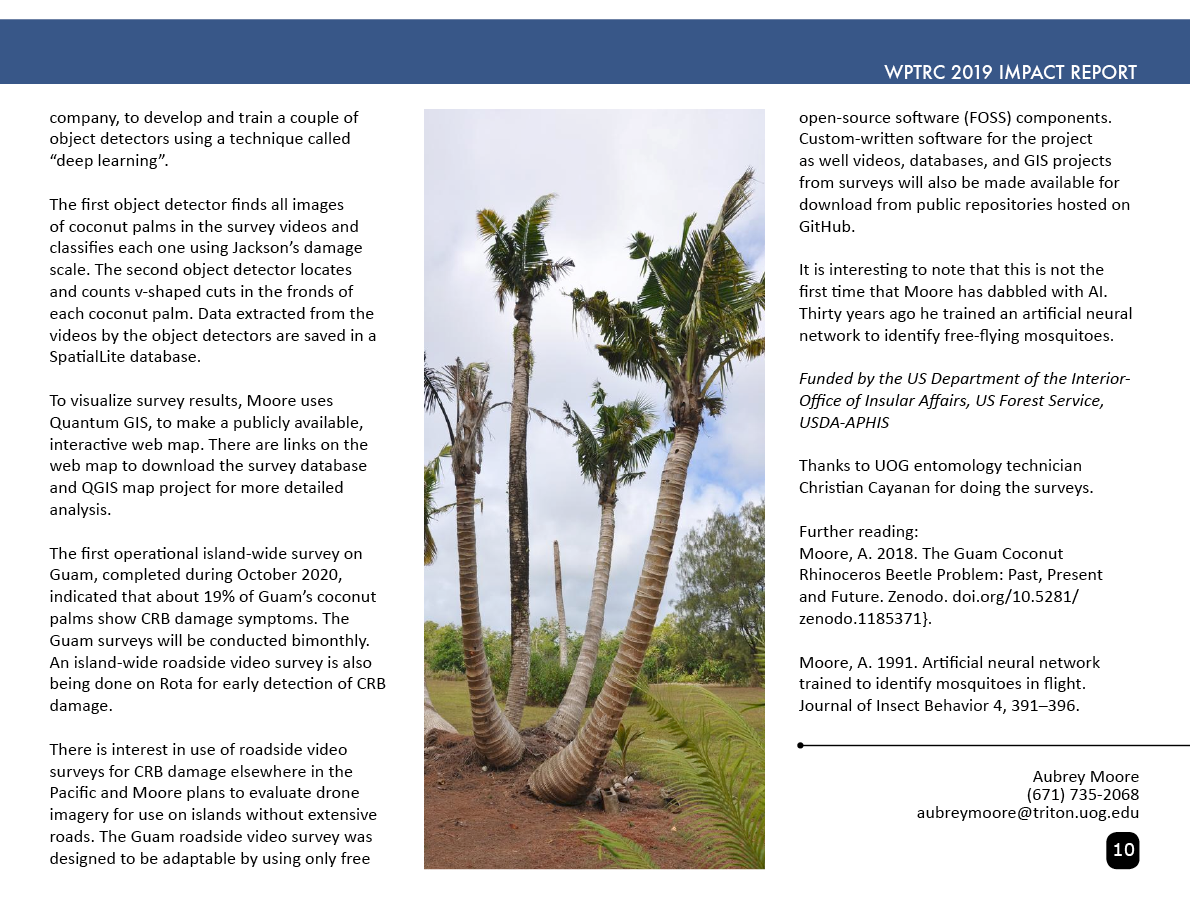
\includegraphics[width=1\linewidth]{images/impact-report10.png}
%	\caption{[Continued] Feature article in the University of Guam's Western Pacific Tropical Research Center impact report for 2020.}
%	\label{fig:roadside1-4}
%\end{figure}
%
%\clearpage
%\paragraph{Guam Roadside Video Survey 2}
%
%The proportion of coconut palms damaged by CRB increased significantly from 19.2\% in
%October 2020 to 21.5\% in December 2020 (p < 0.001; Fisher's exact test).
%
%%\begin{figure}[h]
%%	\centering
%%	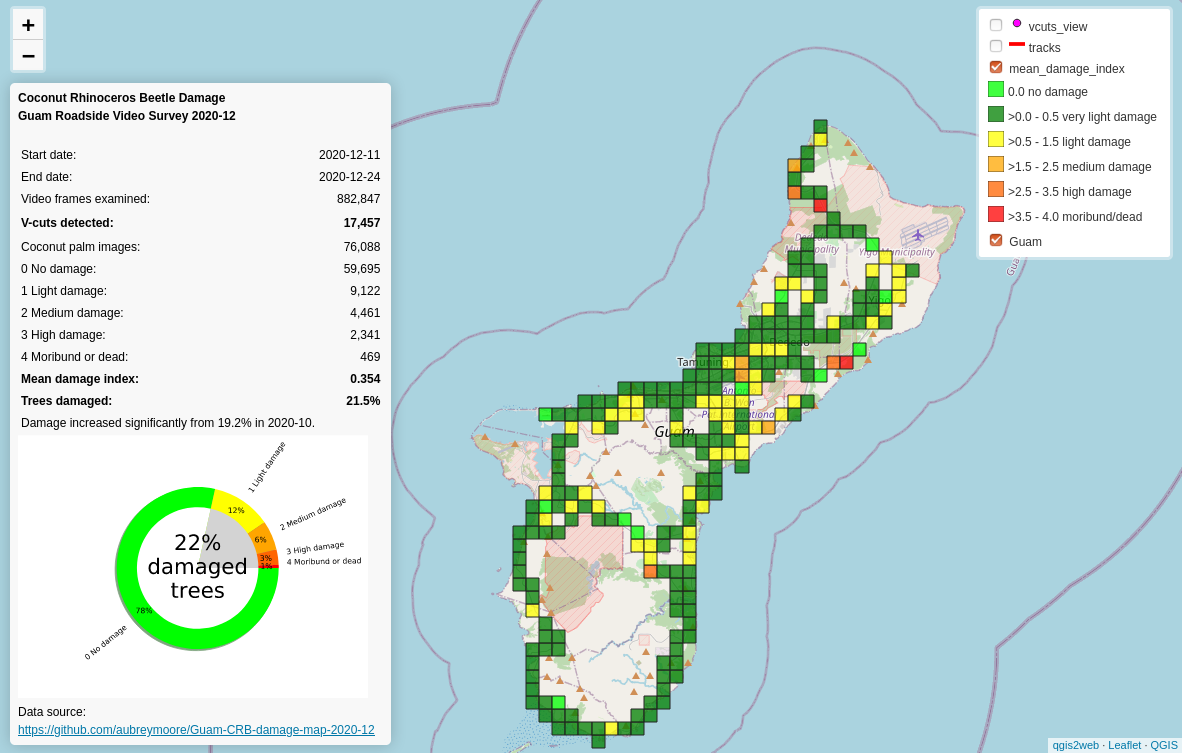
\includegraphics[width=1\linewidth]{../images/crb-webmap-2020-12.png}
%%	\caption{Screenshot of an interactive web map of results from a roadside video survey of
%%		CRB damage on Guam in December 2020 \url{https://aubreymoore.github.io/Guam-CRB-damage-map-2020-12/webmap/v1/}.}
%%	\label{fig:guam02}
%%\end{figure}
%
%
%\clearpage
%\paragraph{Rota Roadside Video Survey 1}
%
%Rota was invaded by CRB in 2017 and eradication efforts by Rota Department of Land and Natural Resources have successfully kept the population at a very low level, although the population has begun to spread to new areas of the island. In October 2020, a smart phone and associated equipment was sent to Rota-DLNR so that they could do an initial roadside video survey in support of their CRB control efforts. In addition to the equipment, a survey setup guide \cite{mooreSetAutomatedRoadside2020} and a setup video \cite{mooreYouTubeVideoMounting2020} were prepared and sent.
% 
%The survey was performed by Mark Mangolana, Rota-DLNR and the phone containing videos from the survey was returned to the University of Guam.  Videos were analyzed using the workflow developed for the Guam surveys. The resulting web map contained many false positives for CRB damage, but there is one hit which shows a classic v-shaped cut probably caused by CRB. For convenience, data for this hit (images, date, location) were documented as an iNaturalist observation (Figure \ref{fig:rota-inat-obs}). If this v-shaped cut was caused by CRB, there will be a bore hole. Rota-DLNR are following up to see if this is the case.
%
%
%\begin{figure}[h]
%	\centering
%	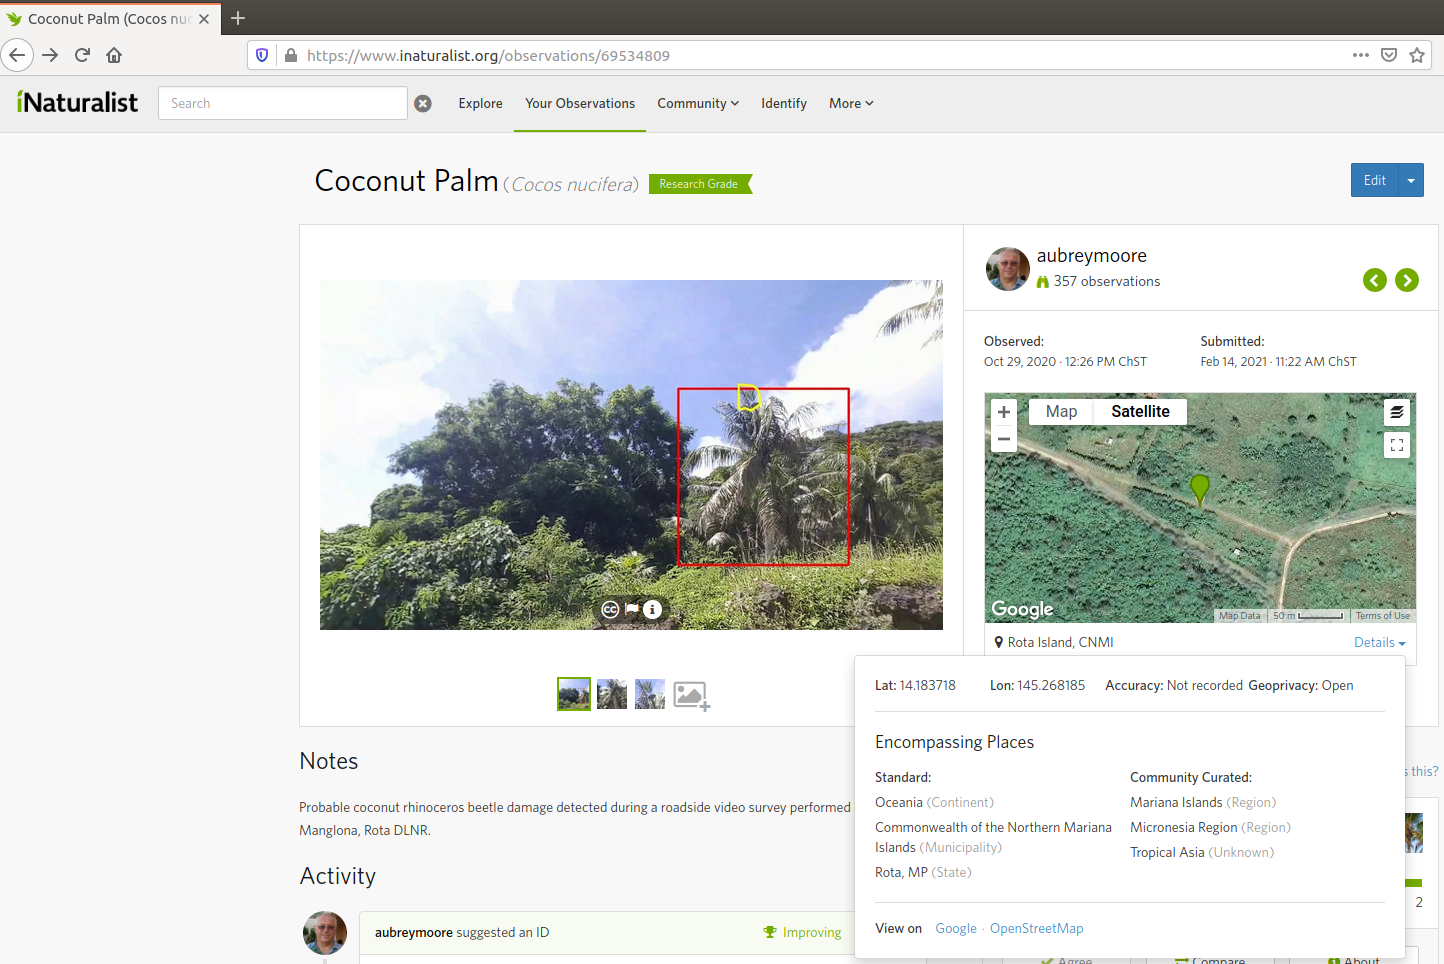
\includegraphics[width=1\linewidth]{images/Rota-iNat-obs}
%	\caption{Screenshot of an iNaturalist observation documenting probable coconut rhinoceros beetle damage detected during a roadside video survey performed by Rota DLNR. \url{https://www.inaturalist.org/observations/69534809}.}
%	\label{fig:rota-inat-obs}
%\end{figure}
%
%\clearpage
%
%\subsubsection{Recent progress}
%
%We continue to monitor CRB damage on Guam using automated roadside image surveys (Fig. \ref{fig:webmap-2021-08} and Fig. \ref{fig:timeline-2021-08}).
%
%We also continue to improve our survey methods. Processing was simplified by changing our raw data format from videos taken at 15 images per second to georeferenced still images taken at 1 image per second. This reduced data file memory requirements by 93\% and we no longer need to rely on a second app to record latitude and longitude.
%
%In addition to using our methods for routine monitoring of CRB damage, they can be used for early detection of CRB. An initial test of this idea was done on Rota and results were reported in a webinar organized by the Depertment of the Interior - Office of Insular Affairs  \cite{usdepartmentoftheinterior-officeofinsularaffairsYouTubeVideoCoconut2021}.
%
%Software tools developed for our automated roadside damage monitoring can be used to detect CRB damage in digital images from any source. Recently, an object detector which we trained to find characteristic v-shaped cuts caused by CRB to examine web images was used to find evidence for an unconfirmed report of CRB establishment in Mexico \cite{jacksonSocialMediaPosts2022}. We were successful (Fig.  \ref{fig:crb-mexico}).
%
%%![](web-screenshot.png)
%%
%%**Figure 1** Screen capture of an online interactive map of coconut rhinoceros beetle damage on Guam. <https://aubreymoore.github.io/Guam-CRB-Damage-Map-2021-08/webmap>
%%
%%![](timeline.pdf)
%%
%%**Figure 2** Changes in CRB damage over time.
%
%% TODO: \usepackage{graphicx} required
%\begin{figure}[H]
%	\centering
%	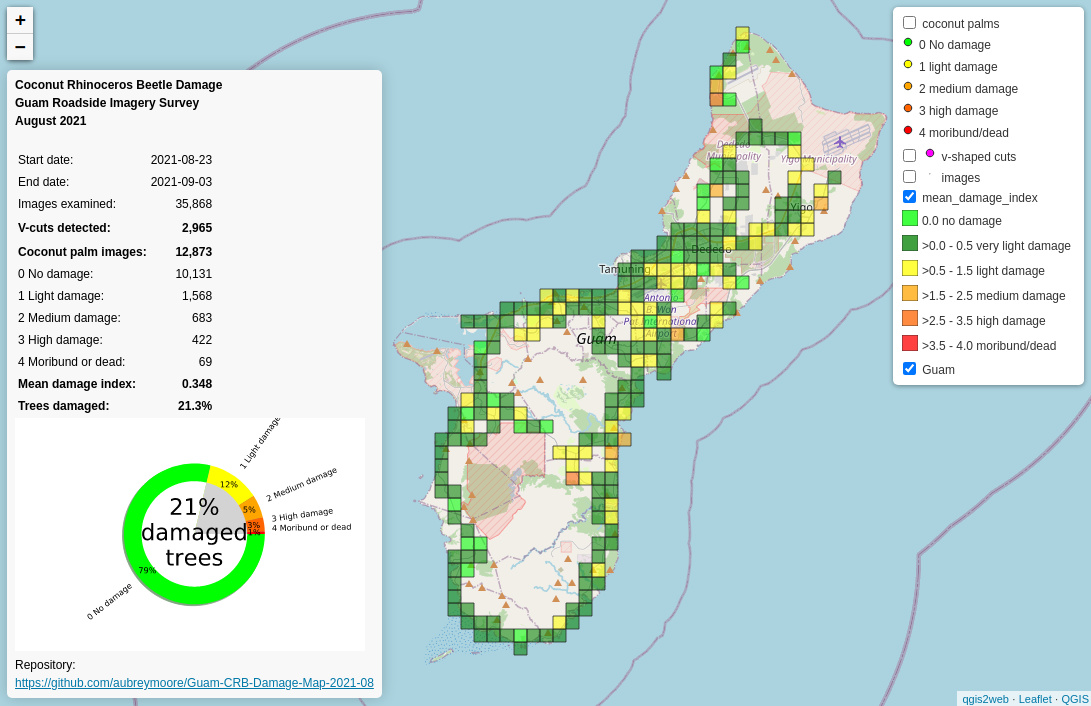
\includegraphics[width=\linewidth]{images/webmap-2021-08}
%	\caption{Screen capture of an online interactive map of coconut rhinoceros beetle damage on Guam. \url{https://aubreymoore.github.io/Guam-CRB-Damage-Map-2021-08/webmap}.}
%	\label{fig:webmap-2021-08}
%\end{figure}
%
%\begin{figure}[H]
%	\centering
%	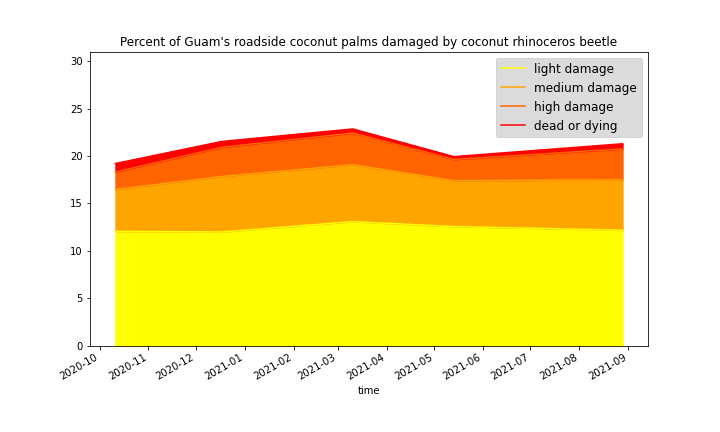
\includegraphics[width=\linewidth]{images/timeline-2021-08}
%	\caption{Changes in CRB damage over time.}
%	\label{fig:timeline-2021-08}
%\end{figure}
%
%\begin{figure}[H]
%	\centering
%	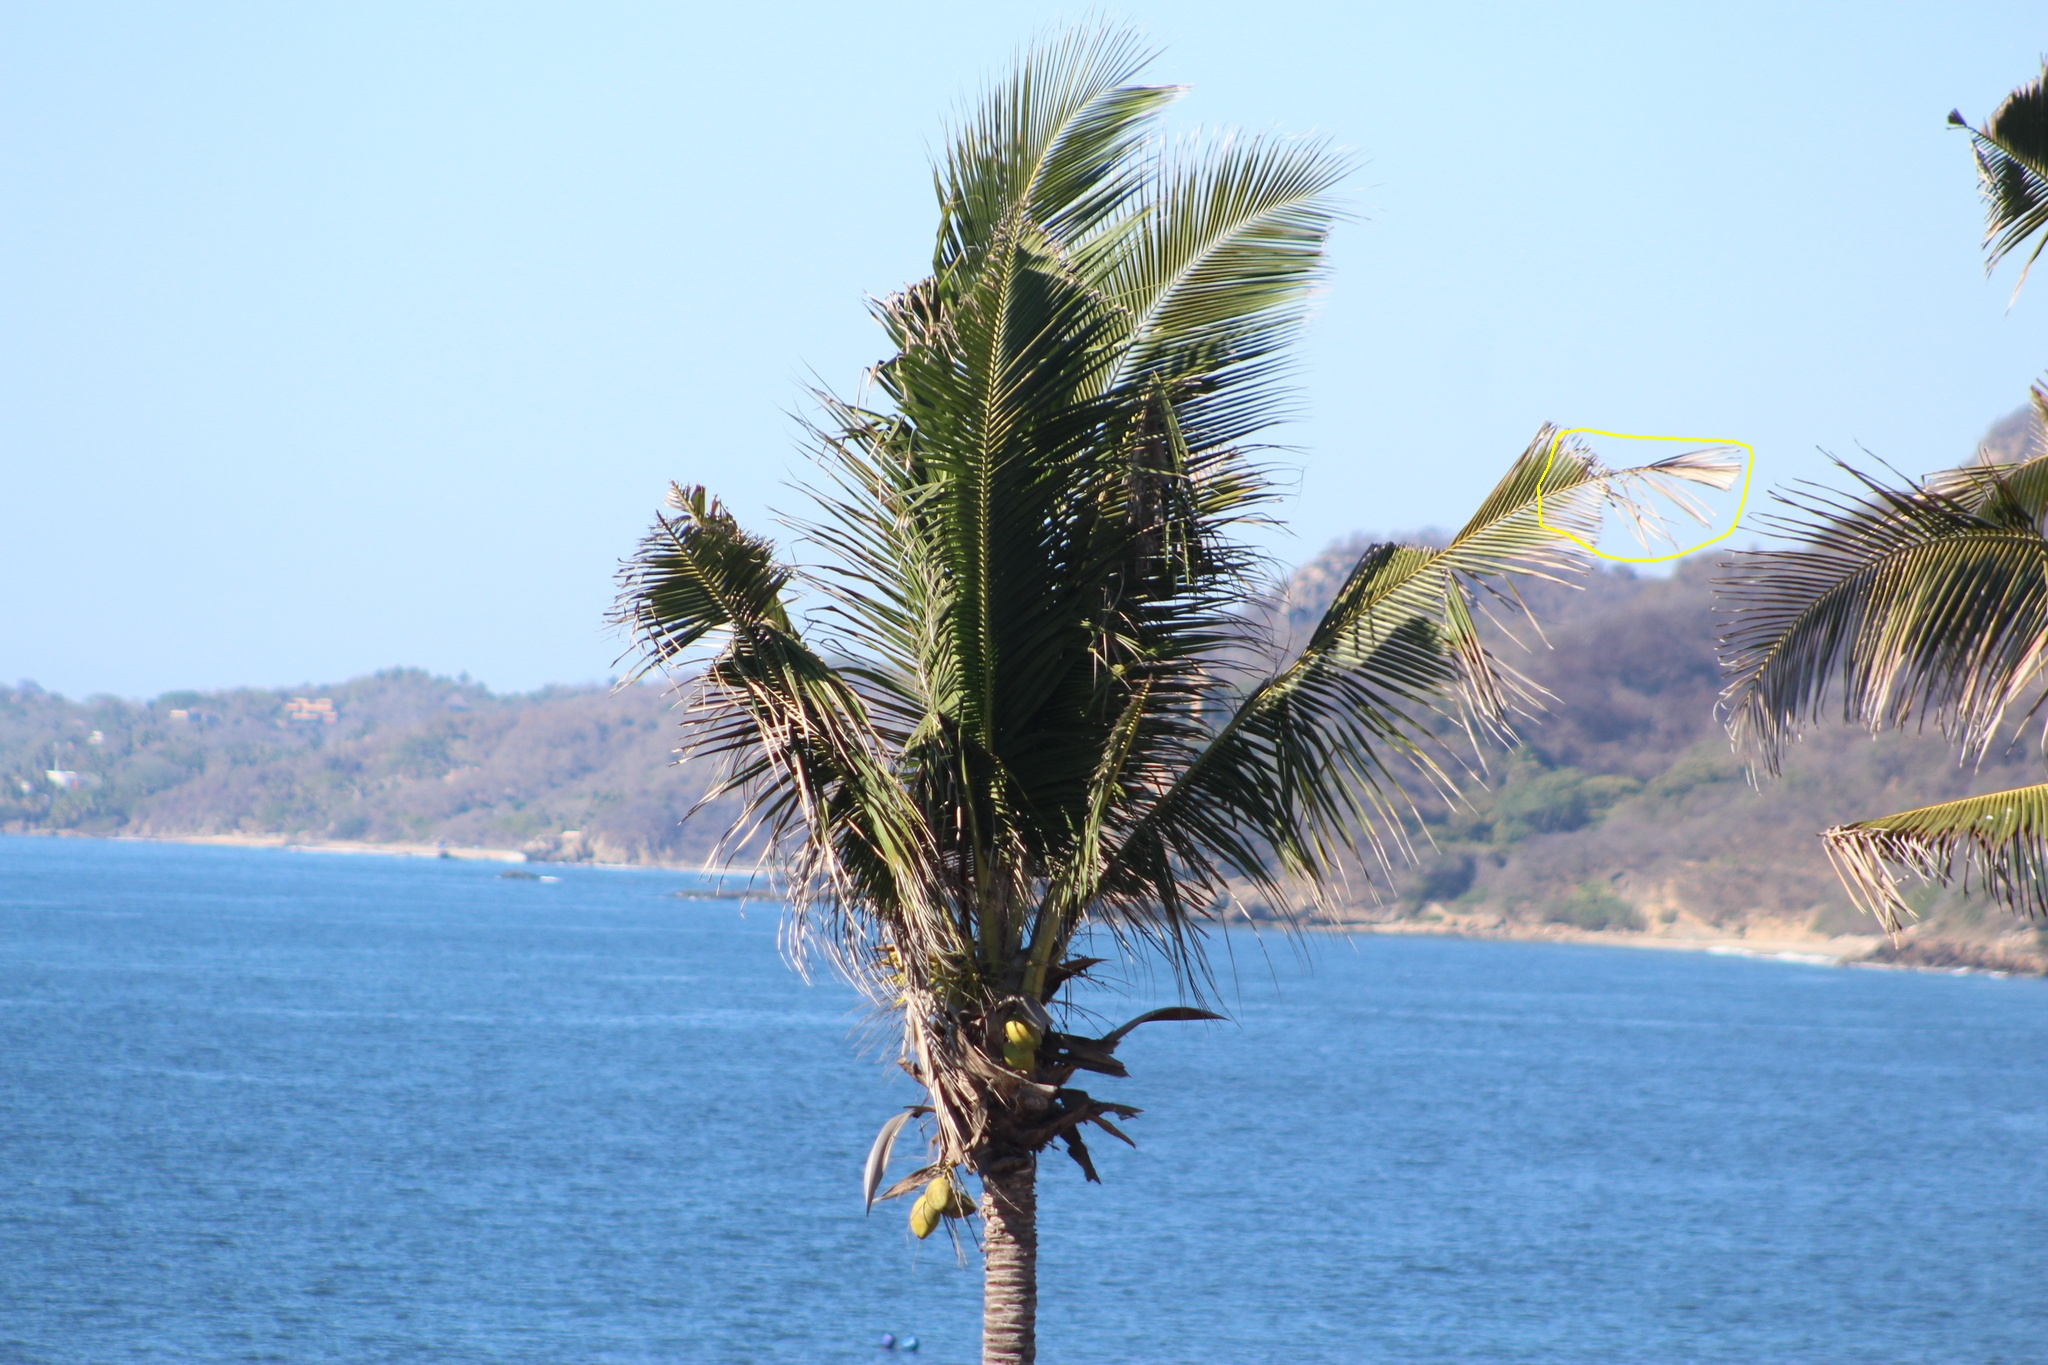
\includegraphics[width=\linewidth]{images/crb-mexico}
%	\caption{Coconut palm in Mexico with CRB damage symptoms. This image was selected by an automated search of web images using an object detector developed for CRB damage monitoring on Guam. Image source: \url{https://www.inaturalist.org/observations/76810823}.}
%	\label{fig:crb-mexico}
%\end{figure}
%
%\clearpage
%
%\section{Related Activities and Recent Progress}
%
%\subsection{Forest Insect and Disease Leaflet (FIDL) for Coconut Rhinoceros Beetle}
%
%The PI is first author on a Forest Service FIDL for CRB (submitted). 

\section{Using Harmonic Radar to Detect CRB Breeding Sites}

Effective control of CRB requires location and destruction of larval breeding sites which my occur anywhere were there is an accumulation of decaying plant material. Previously, we successfully tracked radio-tagged CRB adults to find cryptic breeding sites \cite{moore_judas_2017-1}. But high cost of radio transmitters (about \$200 each) and limited battery capacity make this method too expensive for regular use. 

We suggest that harmonic radar tags may be a cost-effective replacement for miniaturized radio transmitters. Harmonic radar tags do not require a battery, are very inexpensive (about \$4 per tag) and have unlimited shelf and field life. 

US Forest Service funded a field test of this idea based on a small grant proposal  attached as Appendix \ref{appA}. We also published the idea as a journal article \cite{mooreProposalDetectingCoconut2022} attached as Appendix \ref{appB}.

\newpage
\section{Field Test}

In July 2022, Dr. Matt Siderhurst, from Eastern Mennonite University, Virginia and two of his students, Skylar List and and Theodore Yoder, worked with us on Guam to field test the idea of tracking beetles with miniature harmonic radar tags attached to them. We were also assisted by Michael Jordan, US Forest Service.

We used an Open Science Framework project \cite{Moore_Yoder_Cayanan_List_2023} to document this field experiment.

A total of 27 tagged beetles were released at the University of Guam Yigo Experiment Station on July 7 and 11 and 39 beetles were released in Yona on July 12. Surveys using RECCO harmonic radar tranceivers were conducted at Yigo on July 8, 12 and 15 and at Yona on July 13 and 15. No tagged beetles were detected during the 5 surveys.

\begin{table}[!ht]
	\centering
	\caption{caption here}
	\label{table1}
	\begin{tabular}{lcccc}
		\hline
		site & date & total & flew & did not fly \\ \hline
		Yigo & July 7 & 32 & 12 & 20 \\
		Yigo & July 11 & 30 & 19 & 11 \\
		Yona & July 12 & 39 & 33 & 5 \\ \hline
		~ & ~ & 101 & 64 & 36 \\ \hline
	\end{tabular}
\end{table}

\begin{table}[!ht]
	\centering
	\caption{caption here}
	\label{table2}
	\begin{tabular}{lcccc}
		\hline
		site & date & total & wire(s) detached & diode detached \\ \hline
		Yigo & July 7 & 20 & 6 & 0 \\
		Yigo & July 11 & 11 & 11 & 1 \\
		Yona & July 12 & 5 & 5 & 0 \\ \hline
		~ & ~ & 36 & 22 & 1 \\ \hline
	\end{tabular}
\end{table}




Sixty-one percent (22 of the 36) beetles which did not fly had damaged tags: 22 had one or more detached antenna wires and one had a detached diode.

\printbibliography

\newpage
\begin{appendices}

\section{Grant Proposal}
Please see next page.
\label{appA}
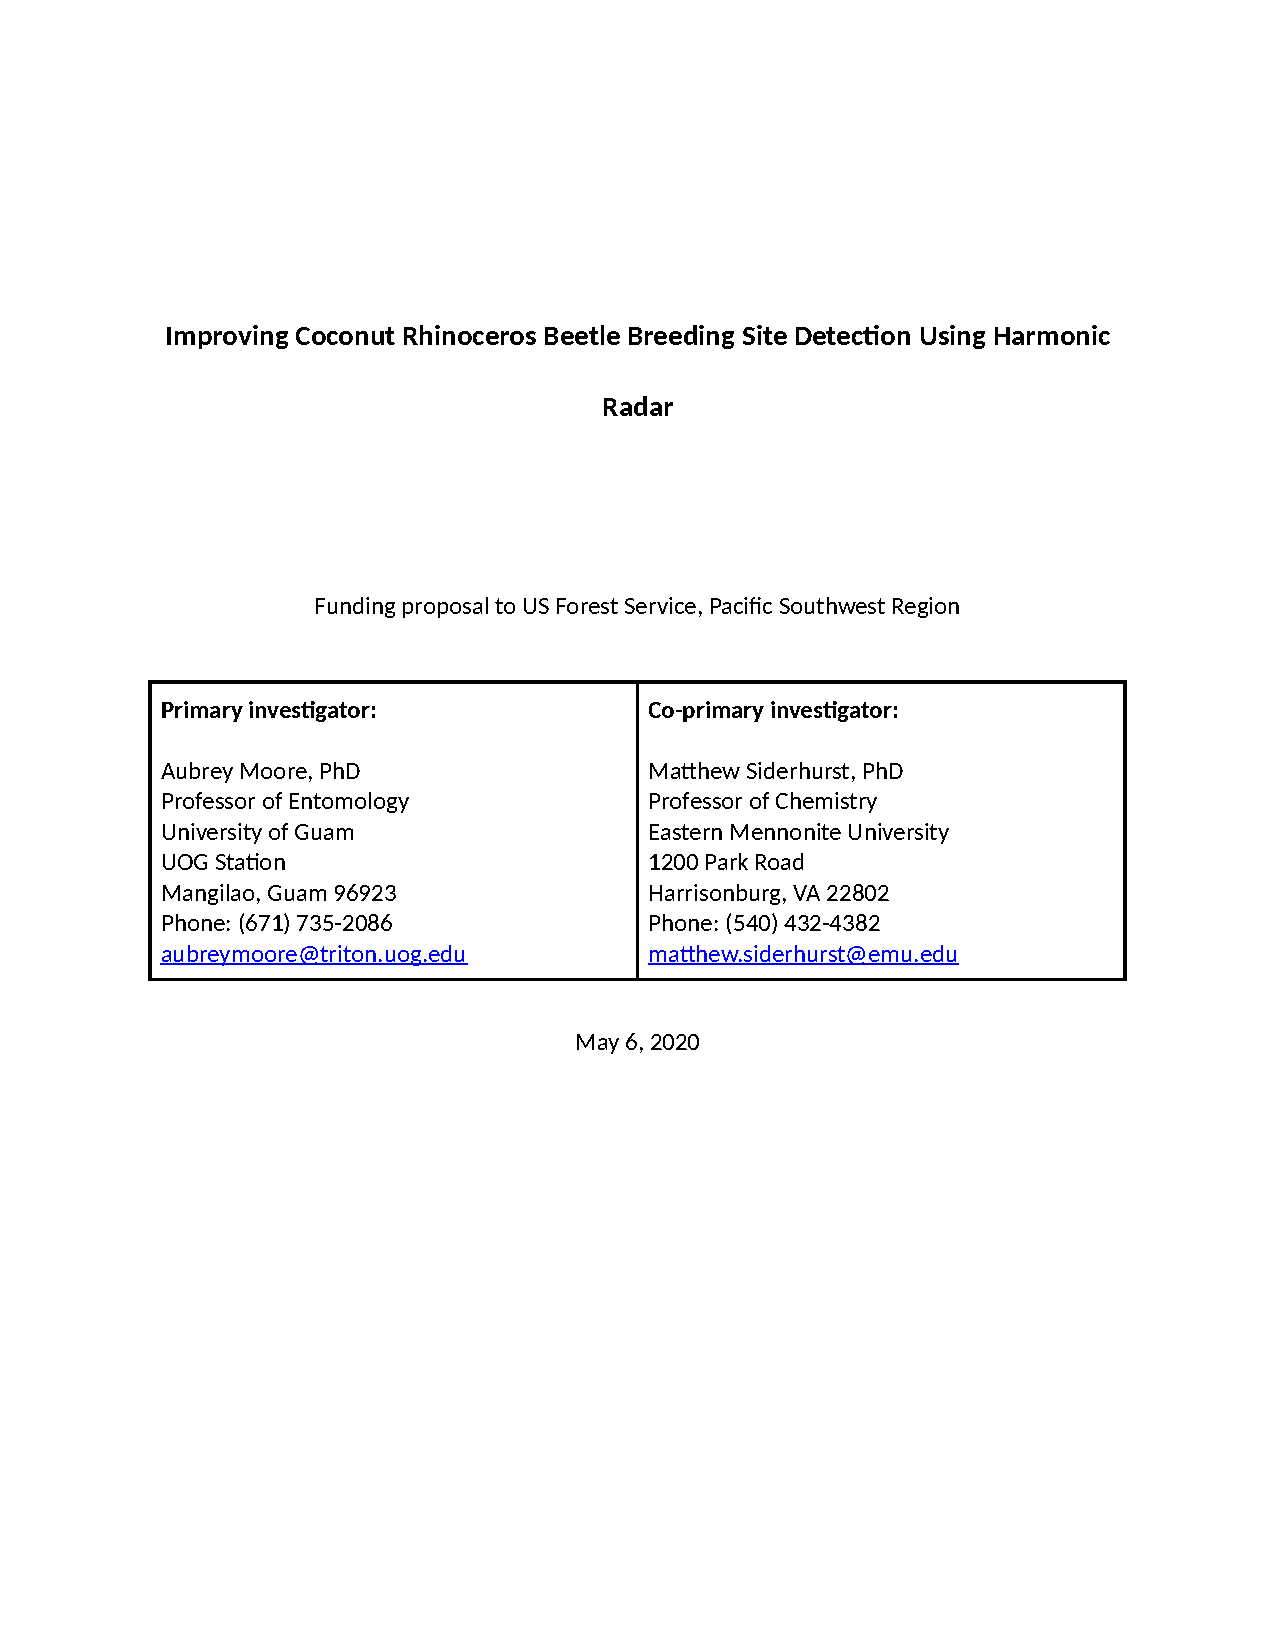
\includepdf[pages=-]{../USFS-harmonic-radar-proposal.pdf}

\newpage
\section{Journal Article}
\label{appB}
Please see next page.
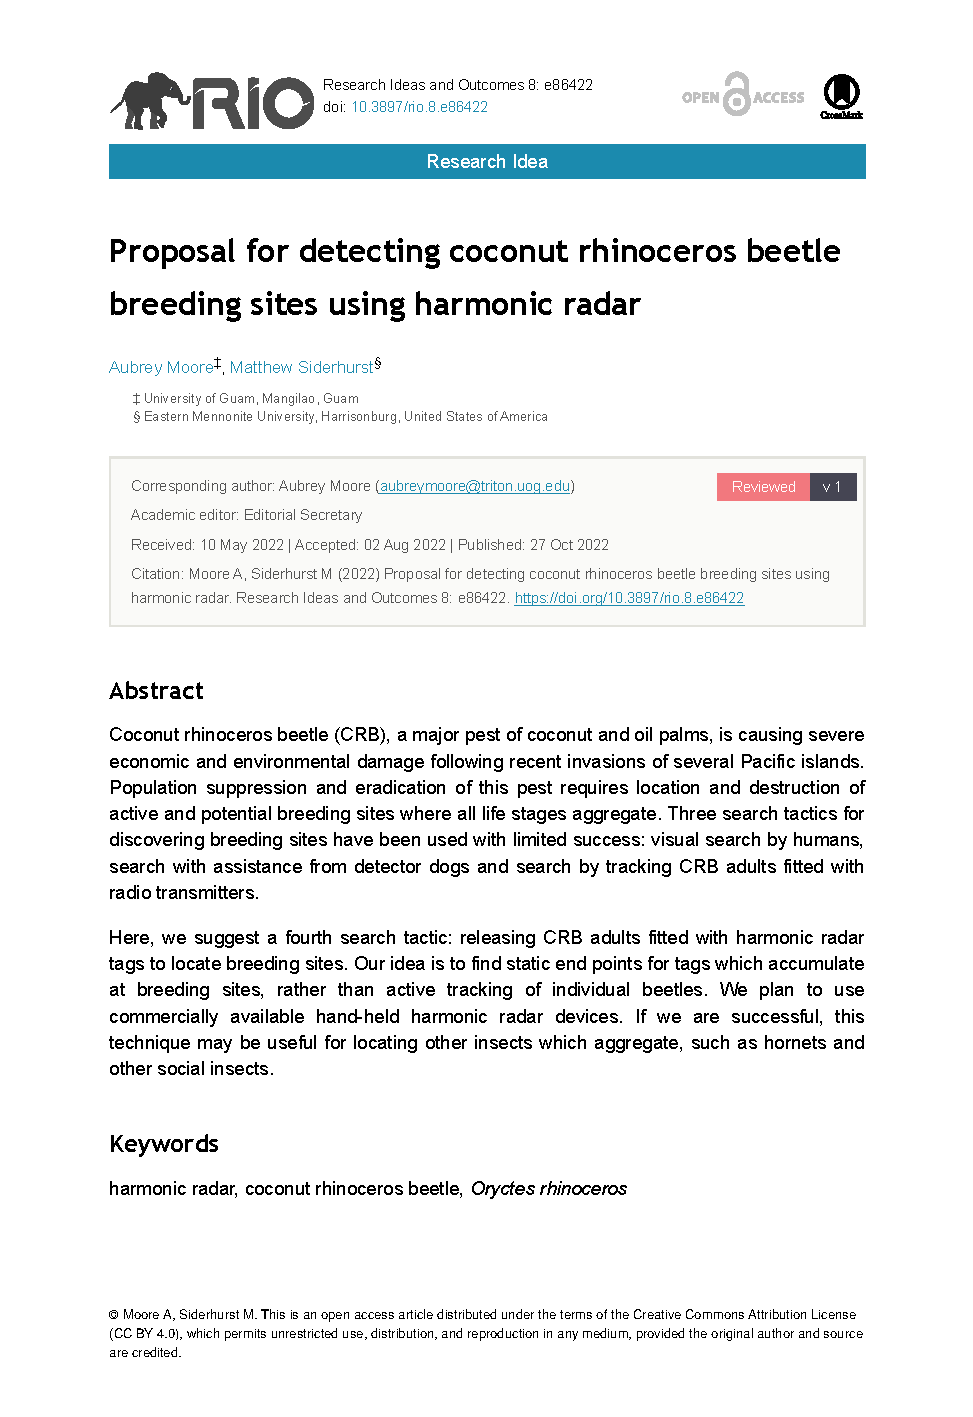
\includepdf[pages=-]{../Moore-and-Siderhurst2022.pdf}

\newpage
\section{Progress Report 4}
\label{appC}
Please see next page.
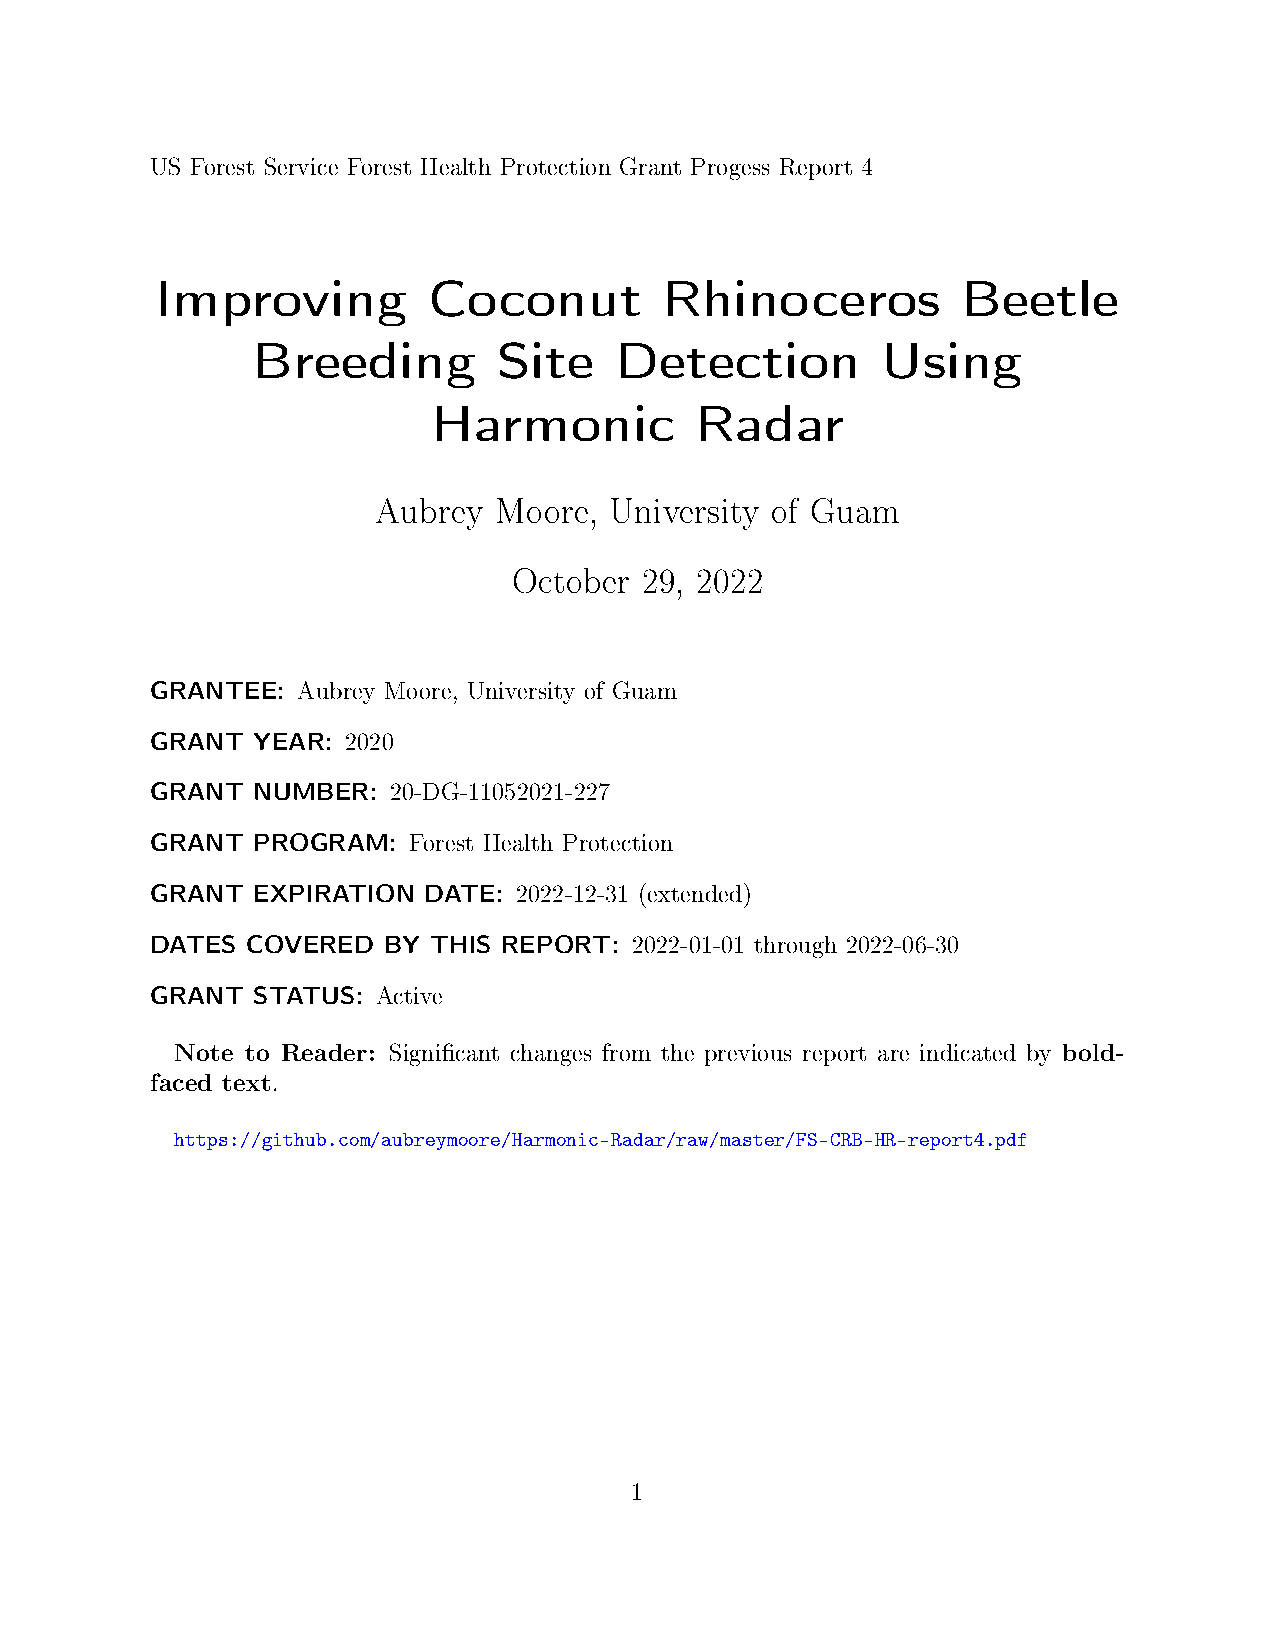
\includepdf[pages=-]{../FS-CRB-HR-report4.pdf}

Please see next page.

\end{appendices}

\end{document}
